
\section{El problema de la mochila}
El problema de la mochila es un clásico en el ámbito de la optimización combinatoria y la teoría de algoritmos. Se trata de seleccionar un subconjunto de artículos, cada uno con un peso y un valor, de manera que se maximice el valor total sin exceder la capacidad de peso permitida. Este problema es fundamental en campos como la logística, la gestión de recursos y la toma de decisiones en la ingeniería. La programación dinámica y las técnicas de aproximación ofrecen métodos eficientes para resolver este problema.

\subsection{Ejemplo 1}
Un naviero tiene un buque carguero con capacidad de hasta 500 toneladas. El carguero transporta contenedores de diferentes pesos para una determinada ruta. En la ruta actual el carguero puede transportar algunos de los siguientes contenedores:

\begin{table}[h!]
\centering
\begin{tabular}{|c|c|c|c|c|c|}
\hline
Contenedor & 1 & 2 & 3 & 4 & 5 \\
\hline
Peso en (cientos de toneladas) & 1 & 2 & 1 & 3 & 4 \\
\hline
Valor (miles de dólares) & 3 & 5 & 4 & 6 & 7 \\
\hline
\end{tabular}
\caption{Datos ejemplo 1}
\end{table}

El analista de la empresa del armador desea determinar el envío (conjunto de contenedores) que maximiza el valor de la carga transportada.

\subsubsection{Código}
\begin{lstlisting}
def algoritmo_mochila(pesos, valores, capacidad):
    n = len(pesos)  
    matriz = []
    for i in range(n + 1):
        fila = []
        for j in range(capacidad + 1):
            fila.append(0)  
        matriz.append(fila)  

    for i in range(1, n + 1):  
        for w in range(1, capacidad + 1):  
            if pesos[i - 1] <= w:  
                matriz[i][w] = max(matriz[i - 1][w], valores[i - 1] + matriz[i - 1][w - pesos[i - 1]])  
            else:
                matriz[i][w] = matriz[i - 1][w]  

    valor_maximo = matriz[n][capacidad]
    return valor_maximo

pesos = [1, 2, 1, 3, 4]  # Pesos en centenas de toneladas
valores = [3, 5, 4, 6, 7]   # Valores en miles de dólares
capacidad = 500              # Capacidad del carguero en toneladas
capacidad_ajustada = capacidad // 100  # Ajustar a centenas
valor_maximo = algoritmo_mochila(pesos, valores, capacidad_ajustada)
print("El valor máximo de la carga transportada es:", valor_maximo, "miles de dólares.")
\end{lstlisting}

\subsubsection{Resultado}
El valor máximo de la carga transportada es: 13 miles de dólares.

\subsubsection{Análisis de complejidad}

\section*{Análisis de Complejidad}

\subsection*{Detalle de Complejidad}

\textbf{1. A: Inicialización de la matriz.}

El código correspondiente es:
\begin{lstlisting}
matriz = []
for i in range(n + 1):  # O(n)
    fila = []
    for j in range(capacidad + 1):  # O(capacidad)
        fila.append(0)  # O(1)
    matriz.append(fila)  # O(1)
\end{lstlisting}

- Inicializar la matriz con ceros tiene una complejidad de \( O(n \times capacidad) \).

\textbf{2. B: Llenado de la matriz con los valores óptimos.}

El código correspondiente es:
\begin{lstlisting}
for i in range(1, n + 1):  # O(n)
    for w in range(1, capacidad + 1):  # O(capacidad)
        if pesos[i - 1] <= w:  # O(1)
            matriz[i][w] = max(matriz[i - 1][w], valores[i - 1] + matriz[i - 1][w - pesos[i - 1]])  # O(1)
        else:
            matriz[i][w] = matriz[i - 1][w]  # O(1)
\end{lstlisting}

- El llenado de la matriz para calcular los valores óptimos tiene una complejidad de \( O(n \times capacidad) \).

\textbf{3. C: Determinación del valor máximo.}

El código correspondiente es:
\begin{lstlisting}
valor_maximo = matriz[n][capacidad]  # O(1)
\end{lstlisting}

- La determinación del valor máximo es una operación constante \( O(1) \).

\subsection*{Complejidad Total}

\[
T(n, capacidad) = O(n \times capacidad)
\]

\subsection*{Variables}

\begin{itemize}
    \item \( n \) = número de artículos.
    \item \( capacidad \) = capacidad de la mochila en centenas de toneladas.
\end{itemize}

\subsection{Ejemplo 2}
Una empresa de transporte marítimo de mercancías posee un barco con una bodega cuya capacidad es de 250 cm³. Desea transportar cuatro bienes de los que se dispone su volumen y su valor monetario. En la siguiente tabla se muestra dicha información:

\begin{table}[H]
    \centering
    \begin{tabular}{cccc}
        \toprule
        \textbf{Bienes} & \textbf{Volumen (cm\(^3\)/Tm)} & & \textbf{Ingresos (\$)} \\
        \midrule
        1 & 70 & & 1250 \\
        2 & 50 & & 900 \\
        3 & 60 & & 1000 \\
        4 & 75 & & 1200 \\
        \bottomrule
    \end{tabular}
    \caption{Datos del problema de la mochila. Elaboración propia.}
    \label{tab:datos_problema}
\end{table}

Se trata de determinar los bienes que se deben transportar en cada bodega de forma que el ingreso sea máximo.

\subsubsection{Código}
\begin{lstlisting}[language=Python]
def mochila(capacidad, volumenes, ingresos, n):
    # Crear una matriz para almacenar los ingresos maximos posibles
    dp = [[0 for x in range(capacidad + 1)] for x in range(n + 1)]

    # Llenar la matriz dp de manera ascendente
    for i in range(n + 1):
        for w in range(capacidad + 1):
            if i == 0 or w == 0:
                dp[i][w] = 0
            elif volumenes[i - 1] <= w:
                dp[i][w] = max(ingresos[i - 1] + dp[i - 1][w - volumenes[i - 1]], dp[i - 1][w])
            else:
                dp[i][w] = dp[i - 1][w]

    # Recuperar los elementos seleccionados
    res = dp[n][capacidad]
    w = capacidad
    bienes_seleccionados = []

    for i in range(n, 0, -1):
        if res <= 0:
            break
        if res == dp[i - 1][w]:
            continue
        else:
            bienes_seleccionados.append(i - 1)
            res -= ingresos[i - 1]
            w -= volumenes[i - 1]

    # Crear una lista que indique si cada bien se lleva (1) o no (0)
    seleccion = [0] * n
    for i in bienes_seleccionados:
        seleccion[i] = 1

    return dp[n][capacidad], bienes_seleccionados, seleccion

# Datos del problema
volumenes = [70, 50, 60, 75]
ingresos = [1250, 900, 1000, 1200]
capacidad = 250
n = len(volumenes)

# Resolver el problema
ingreso_maximo, bienes_seleccionados, seleccion = mochila(capacidad, volumenes, ingresos, n)

print(f"El ingreso maximo es: ${ingreso_maximo}")
print("Bienes seleccionados (indices):", bienes_seleccionados)
print("Seleccion de bienes (1 = seleccionado, 0 = no seleccionado):")
for i in range(n):
    print(f"Bien {i + 1}: {seleccion[i]}")
\end{lstlisting}

\subsubsection{Resultado}
\begin{figure}[H]
    \centering
    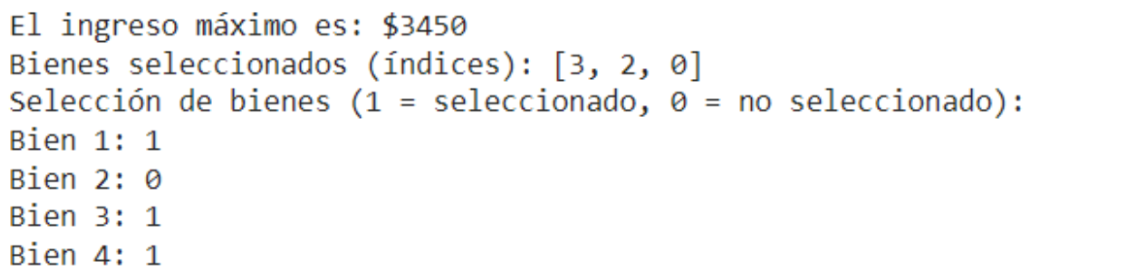
\includegraphics[width=0.8\textwidth]{resultado_mochila_ejem2.png}
    \caption{Imagen del resultado del código Python.}
    \label{fig:resultado_ejemplo2}
\end{figure}

\subsubsection{Análisis de complejidad}
\begin{figure}[H]
    \centering
    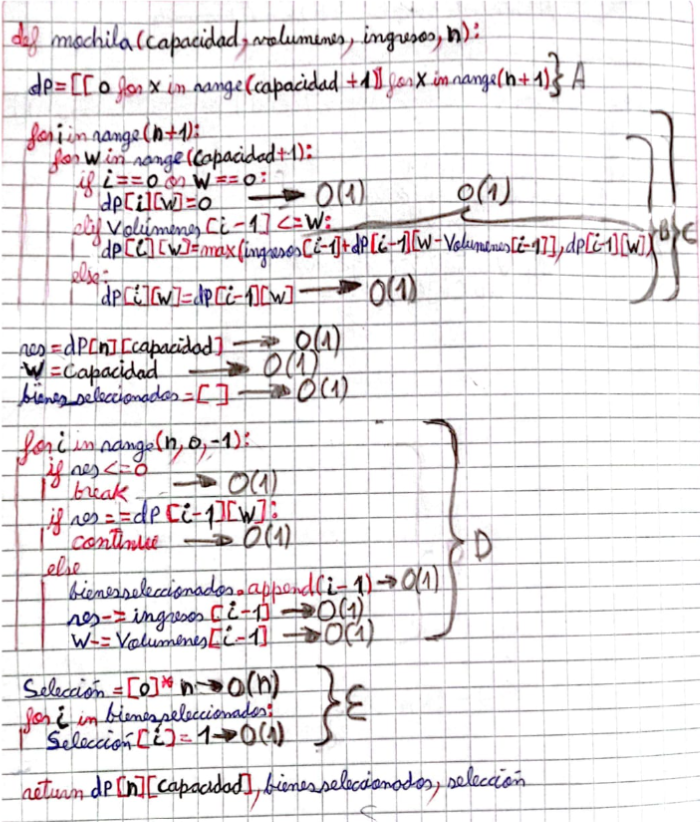
\includegraphics[width=0.8\textwidth]{complejidad_mochila_ejem2.png}
    \caption{Análisis del código.}
    \label{fig:complejidad_ejemplo2}
\end{figure}

\begin{figure}[H]
    \centering
    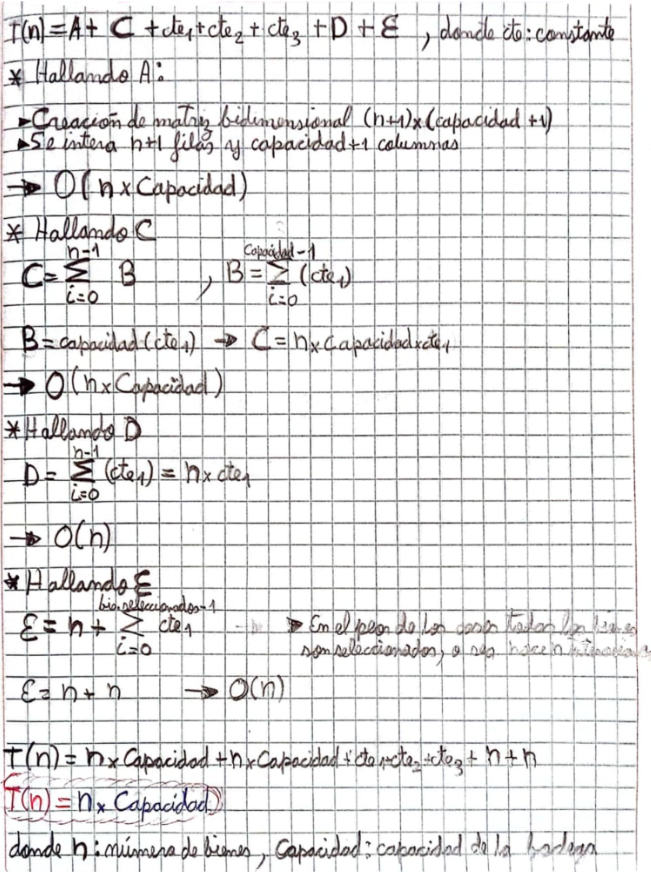
\includegraphics[width=0.8\textwidth]{complejidad_mochila_ejem2_2.png}
    \caption{Análisis del código.}
    \label{fig:complejidad_ejemplo2_2}
\end{figure}

Como se acaba de apreciar, el presente algoritmo tiene una complejidad aproximada de O(n x K) o, equivalentemente, n x capacidad, lo cual supone eficiencia en función al dato de entrada de “capacidad”; mientras más sea esto, más complejo se vuelve.
